\documentclass[a4paper,15pt]{article}
\usepackage{enumerate}
\usepackage{graphicx}
\usepackage{algorithm2e}
\usepackage{amsmath}
\usepackage{multirow}

\title{LaTex Programs}
\author{NAYAKANTI SAI MIHIRNATH}
\date{December 2022}

\begin{document}
	\maketitle
	\pagebreak
	\tableofcontents
	\newpage
	\section{Introduction}
	Welcome to Practice Session
	\paragraph{Avengers : }
	\subparagraph{Avengers , a main part of Marvel Cinematic Universe}
	\subparagraph{Ironman , Captain America , Hulk , Spiderman}
	\subsection{LaTeX}
	LaTex Programs
	\subsubsection{Doc}
	Article and Report
	\newpage
	\section{Unordered List}
	\begin{itemize}
		\item Ironman
		\item Captain America
		\item Hulk
		\item Hawkeye
		\item Captain Marvel
	\end{itemize}
	\section{Ordered List}
	\begin{enumerate}[(i)]
		\item Spiderman
		\item America Chavez
		\item She Hulk
		\item Ms Marvel
		\item Ant Man
	\end{enumerate}
	\pagebreak
	\section{Nested List}
	\begin{itemize}
		\item[$*$] Avengers
		\begin{enumerate}[(I)]
			\item Ironman
			\item Captain America
			\item Hulk
			\item Hawkeye
			\item Captain Marvel
		\end{enumerate}
		\item[Note:] Harry Potter Characters
		\begin{enumerate}
			\item Harry Potter
			\item Hermione Granger
			\item Ron Weasley
			\item Draco Malfoy
			\item Albus Dumbledore
			\item Severus Snape
			\item Tom Riddle
		\end{enumerate}
		\item[!] Star Wars episodes:
		\begin{enumerate}[I:]
			\item The Phantom Menace
			\item Attack of the Clones
			\item Revenge of the Sith
			\item A New Hope
			\item The Empire Strikes Back
			\item Return of the Jedi
			\item The Force Awakens
		\end{enumerate}
	\end{itemize}
	\newpage
	\section{Image}
	\begin{figure}[h!bt]
		\centering
		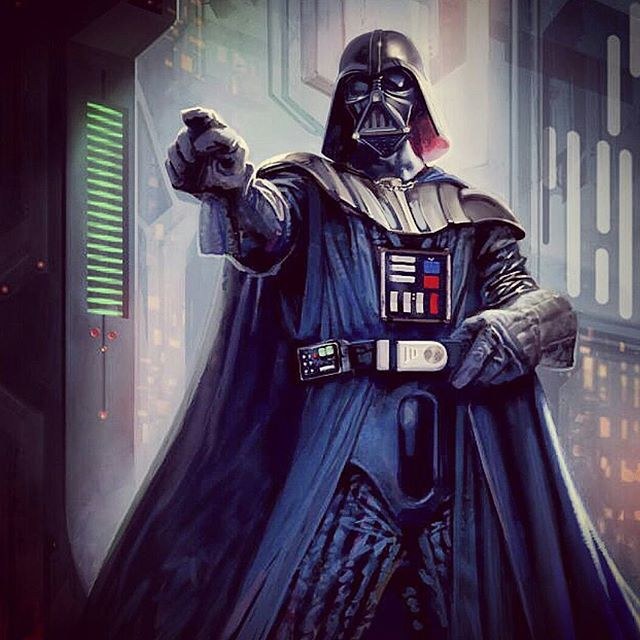
\includegraphics[width=\textwidth]{DarthVader.jpg}
		\caption{Darth Vader}
		\label{Darth Vader}
	\end{figure}
	\newpage
	\section{Tables}
	\begin{tabular}{|c|c|cc|}
		\hline
		\textbf{Name} & \textbf{Phone Number} & \multicolumn{2}{c}{\textbf{Address}} \\
		\hline
		Mihir & 7673916996 & & \\
		\cline{1-2}
		Hruthik & 6300961913 & & \\
		\cline{1-2}
		\multirow{2}{*}{Dark Lord} & & & \\
		\cline{2-2}
		& & & \\
		\hline
	\end{tabular}
\end{document}
